%!TEX root = main.tex

\chapter{Procesos Gaussianos Deformados}
\label{sec:cwgp}

\begin{chapquote}{George Box}
	``...todos los modelos son aproximaciones. Esencialmente, todos los modelos son incorrectos, pero algunos son útiles. Sin embargo, siempre se debe tener en cuenta la naturaleza aproximada del modelo.''
\end{chapquote}

\comment{esta es una wena intro de capitulo!}

En este capítulo, nuestra motivación inicial es extender el marco de los procesos gaussianos \cite{rasmussen06} del capítulo \ref{sec:gaussian} para incluir procesos no gaussianos y para ser más preciso en las suposiciones que relativas a los datos modelados. Para lograr esto, primero, en la sección \ref{sec:wgp} revisaremos un modelo generativo para procesos no gaussianos, llamados procesos gaussianos deformados (WGP por sus siglas en inglés, \emph{warped Gaussian processes}) \cite{snelson2004warped}, en donde a un proceso gaussiano latente se le aplica (coordenada a coordenada) una transformación no lineal expresiva e \emph{invertible}, llamada \emph{deformación}. La mayor contribución de este capítulo es el modelo que se propone en la sección \ref{sec:novelWGP}, el llamado proceso gaussiano deformado por composiciones (CWGP por sus siglas en inglés, \emph{compositionally-warped GP}) \cite{riostobar2019cwgp}, es decir, un WGP en donde la función de deformación es la composición de funciones elementales. Al escoger funciones elementales que tienen derivadas e inversas con fórmula cerrada, este modelo requiere aproximaciones numéricas mínimas, logrando una complejidad computacional atractiva para poder predecir y aprender. En la sección \ref{sec:transformations} describimos un conjunto ad hoc de funciones elementales con fórmulas explícitas para sus derivadas e inversas, y destacamos sus propiedades y una recomendación de cómo usarlas, descritas en la sección \ref{sec:choice_trans}. Para concluir este capítulo, en la sección \ref{sec:experiments} damos ejemplos ilustrativos usando datos sintéticos y reales, que validan el método propuesto versus un WGP en términos de replicabilidad, eficiencia computacional y habilidad predictiva.

%\fbox{\begin{minipage}{39.5em}
%		\scriptsize	
%		The results presented in this Chapter correspond to them in two published papers \cite{rios2018learning,riostobar2019cwgp}: 1) \emph{Gonzalo Rios and Felipe Tobar. Learning non-Gaussian time series using the Box-Cox Gaussian process. In International Joint Conference on Neural Networks, 2018}, and
%		2) \emph{Gonzalo Rios and Felipe Tobar. Compositionally-warped Gaussian processes. Neural Networks, 118:235-246, 2019}.
%\end{minipage}}

A pesar de los hechos a favor de la distribución gaussiana presentada en el capítulo \ref{sec:gaussian}, la suposición de la gaussianidad conjunta está lejos de ser real en muchos contextos. En la práctica, uno se enfrenta con observaciones que no son simétricas, que tienen colas pesadas, o que están acotadas por alguna restricción física o económica. Todas estas propiedades se contradicen con el margo gaussiano. Por ejemplo, en la presencia de observaciones estrictamente positivas, como precios de una moneda o el flujo de un río, suponer la propiedad de gaussianidad es un error, pues la distribución gaussiana tiene soporte en toda la línea real. Esto nos motiva a estudiar modelos que posean las propiedades atractivas de los procesos gaussianos, pero con hipótesis más flexibles sobre los fenómenos modelados.

\begin{figure}[h]
	\centering
	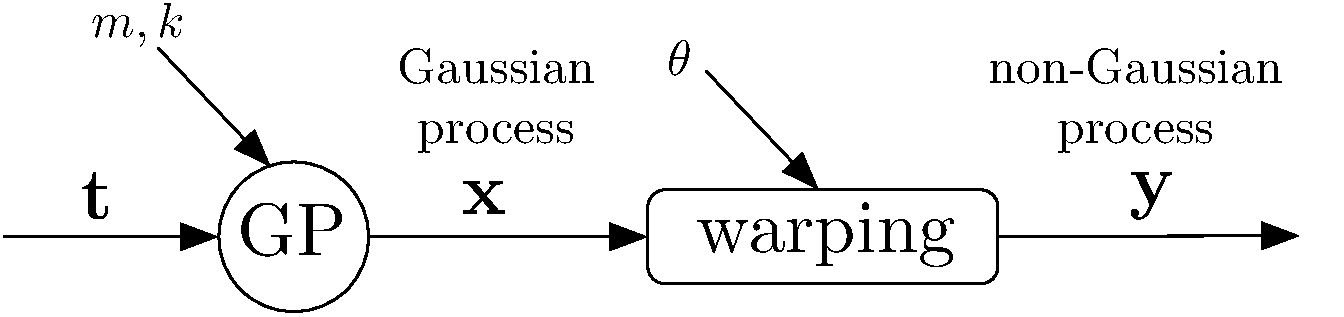
\includegraphics[width=0.6\textwidth]{wgp}
	\caption{Estructura general de los procesos gaussianos deformados, donde se transforma de manera no lineal un GP para modelar observaciones no gaussianas.}
	\label{fig:wgp}
\end{figure}

Para modelar datos no gaussianos y mantener el uso de las ventajas de los modelos gaussianos, uno puede transformar los datos observados \(\bfy \in \calY^N\) vía una biyección no lineal y diferenciable \(\varphi : \calY \to \calX\), llamada \emph{deformación}, tal que \(\bfx = \Phi(\bfy) = [\varphi(y_1), \dotsc, \varphi(y_N)]^\top\) es \emph{más gaussiano} y puede ser modelado como un GP (ver la Figura \ref{fig:wgp}). Este enfoque es estándar en estadística, donde es usual escoger como función a \(\varphi(y) = \log(y)\), en donde se supone implícitamente que el proceso observado tiene marginales log-normales, así que el fenómeno modelado toma valores positivos.

Como la transformación \(\Phi\) es diagonal desde un punto de vista coordenada a coordenada, las distribuciones transformadas satisfacen las condiciones del Teorema de Consistencia de Kolmogorov \cite{tao2011introduction} (introducido en la sección \ref{sec stochastic process}). Dicho modelo generativo es un proceso no gaussiano llamado proceso gaussiano deformado \cite{snelson2004warped}. En la sección \ref{sec:marginaltransport} demostraremos esta proposición de forma más general, así que la consideraremos como cierta por el resto de este capítulo.

Nuestro objetivo es construir una nueva deformación para procesos gaussianos que herede la expresividad de las estructuras más profundas, pero que a la vez requiera aproximaciones numéricas mínimas para poder predecir. Esto se logrará al construir deformaciones que tengan inversas conocidas y con fórmula cerrada.

\section{El Teorema del Cambio de Variables}

\comment{este va aca o en el marco teorico??}
Una manera estándar de abordar el modelamiento de observaciones no gaussianas es transformar los datos usando funciones como el logaritmo \cite{boxcox} o la tangente hiperbólica \cite{johnsonsu}, de forma tal que los datos transformados se distribuyan de forma normal (o estén cerca de hacerlo). Esta transformación resulta en un cambio de la medida de probabilidad \cite{tao2011introduction}, en donde la distribución de la variable transformada, dada la transformación, se conoce explícitamente. Sin embargo, usualmente este resultado y sus implicancias teóricas en la construcción de modelos no gaussianos expresivos son ignorados. Presentamos formalmente el cambio de medida de probabilidad que resulta de transformar una variable aleatoria vía el siguiente teorema, para luego estudiar el caso gaussiano.

\begin{theorem}[Cambio de Variables Probabilístico \cite{hogg1995introduction}]
	\label{thm:CoV}
	Sea \(\bfx \in \calX \subseteq \reals^{n}\) un vector aleatorio con una función de densidad de probabilidad dada por \(p_{\bfx}(\bfx)\), y sea \(\bfy \in \calY \subseteq \reals^n\) un vector aleatorio tal que \(\varphi(\bfy) = \mathbf{x}\), en donde la función \(\varphi : \calY \to \calX\) es biyectiva, de clase \(\calC^{1}\), y \(\vert \nabla \varphi(\bfy) \vert > 0\) para todo \(\bfy \in \calY\). Entonces, la función de densidad de probabilidad \(p_\bfy\) inducida en \(\calY\) está dada por
	\begin{equation*}
		p_{\bfy}(\bfy) = p_{\bfx}(\varphi(\bfy)) \vert \nabla \varphi(\bfy)\vert,
	\end{equation*}
	donde \(\nabla \varphi\) denota al jacobiano de \(\varphi\), y \(\vert \cdot \vert\) denota a la función determinante.
\end{theorem}

Diremos que \(\bfx = [x_{1}, \dotsc, x_{n}]^\top\) son las variables \emph{basales} y que \(\bfy = [y_{1}, \dotsc, y_{n}]^\top\) son las variables \emph{transformadas}. El teorema de cambio de variables nos da una metodología para expresar la función de densidad de probabilidad (f.d.p.) de las variables transformadas en términos de (a) la f.d.p. de las variables basales y (ii) la transformación aplicada.

Como nuestro objetivo es usar el teorema de cambio de variables para construir modelos no gaussianos que sean manejables, consideremos un vector aleatorio normal multivariado \(\bfx \in \reals^n\) con media \(\mu_{\bfx}\) y covarianza \(\Sigma_{\bfx}\), denotado \(\bfx \sim \calN(\mu_{\bfx}, \Sigma_{\bfx})\), y, además, un mapeo coordenada a coordenada\footnote{Para simplificar la notación, denotaremos a los mapeos vectoriales o escalares por \(\varphi\) indistintamente.} desde el espacio transformado al espacio basal dado por
\begin{equation*}
	\bfy \mapsto \bfx = \varphi(\bfy) = [\varphi(y_{1}), \dotsc, \varphi(y_{n})]^\top.
\end{equation*}
Notemos que el jacobiano de \(\varphi(\bfy)\) es diagonal y, por ende, podemos factorizar su determinante como
\begin{equation*}
	\vert \nabla \varphi(\bfy) \vert = \prod_{i=1}^{n} \dv{\varphi(y_{i})}{y} > 0.
\end{equation*}
En este contexto, podemos obtener explícitamente la f.d.p. de \(\bfy = [y_1, \dotsc, y_N]^\top\) usando el teorema \ref{thm:CoV}, y tiene la forma
\begin{equation*}
	p(\bfy) = \prod_{i=1}^{n} \dv{\varphi(y_{i})}{y} \calN(\varphi(\bfy) \mid \mu_{\bfx}, \Sigma_{\bfx}),
\end{equation*}
en donde la función \(\varphi\) es afín si y solo si la distribución \(p(\bfy)\) es gaussiana. Cabe destacar que la distribución \(p(\bfy)\) en general no es gaussiana, pero está parametrizada por la media basal \(\mu_{\bfx}\), la varianza basal \(\Sigma_{\bfx}\) y la transformación\(\varphi\).

También podemos usar el teorema \ref{thm:CoV} para calcular las densidades condicionales de vectores aleatorios gaussianos transformados: para dos vectores conjuntamente gaussianos \(\bfx, \bfx'\) con densidades condicionales \(p(\bfx \mid \bfx') = \calN(\mu_{\bfx \mid \bfx'}, \Sigma_{\bfx \mid \bfx'})\), y un par de vectores \(\bfy, \bfy'\) tales que \(\bfx = \varphi(\bfy)\) y \(\bfx' = \varphi(\bfy')\), la densidad condicional \(p(\bfy \mid \bfy')\) está dada por
\begin{align*}
	p(\bfy \mid \bfy')			&= \prod_{i=1}^{n} \dv{\varphi(y_{i})}{y} \calN(\varphi(\bfy) \mid \mu_{\bfx \mid \bfx'}, \Sigma_{\bfx \mid \bfx'})\\
	\mu_{\bfx \mid \bfx'}		&= \mu_{\bfx} + \Sigma_{\bfx \bfx'} \Sigma_{\bfx' \bfx'}^{-1} (\varphi(\bfy') - \mu_{\bfx'})\\
	\Sigma_{\bfx \mid \bfx'}	&= \Sigma_{\bfx \bfx} - \Sigma_{\bfx \bfx'} \Sigma_{\bfx' \bfx'}^{-1} \Sigma_{\bfx' \bfx},
\end{align*}
donde recordemos que \(\Sigma_{\bfx \bfx'}\) denota la covarianza entre \(\bfx\) y \(\bfx'\), y \(\mu_\bfx\) denota la media marginal de \(\bfx\).

Observemos que la densidad posterior del elemento transformado \(p(\bfy \mid \bfy')\) pertenece a la misma familia que la densidad incondicional \(p(\bfy)\). Esta propiedad de cerradura al tomar condicionales se hereda de la f.d.p. gaussiana base, y se preserva al aplicar la transformación por coordenada \(\varphi\). Más aún, la distribución multivariada no gaussiana \(p(\bfy)\) también es cerrada bajo marginalización y permutación, porque (de nuevo) \(\varphi\) se define por coordenada.

Por lo tanto, podemos construir un proceso no gaussiano al \emph{transformar} (o \emph{deformar}) un GP de la siguiente forma: (i) escogemos un GP base \(x\) y una transformación por coordenada \(\varphi\), (ii) calculamos las densidades marginales finito-dimensionales de \(y\) sujeto a que \(x = \varphi(y)\) usando el teorema de cambio de variables, y (iii) aplicamos el teorema de consistencia de Kolmogorov \cite{tao2011introduction}. Esta construcción garantiza la existencia de tales procesos no gaussianos con hiperparámetros conocidos: la media y la covarianza del GP base, y la transformación \(\varphi\).

\section{Procesos Gaussianos Deformados}
\label{sec:wgp}

Los procesos gaussianos deformados (WGP por sus siglas en inglés) \cite{snelson2004warped} siguen la misma base lógica explicada en la sección anterior. Un WGP considera un GP con media cero y una función de covarianza exponencial cuadrática (SE), así como una transformación por coordenada paramétrica monótona (por ende, invertible).

La transformación \(\varphi : \reals \to \reals\) considerada en \cite{snelson2004warped} está dada por
\begin{equation}
	\label{eq:wgp}
	\varphi (y) = y + \sum_{j=1}^{d} a_{j} \tanh(b_{j}(y + c_{j})),
\end{equation}
donde \(a_{j}, b_{j} \geq 0\) para \(j = 1, \dotsc, d\). La mezcla de las funciones de identidad y la tangente hiperbólica en la ecuación \eqref{eq:wgp} actúa como una deformación paramétrica de la función identidad, lo que significa que el WGP no permite las transformaciones estándar, como el logaritmo. Notemos que, dado que \(\varphi(y)\) en la ecuación \eqref{eq:wgp} es una suma de términos monótonos, su inversa existe. Sin embargo, como esta inversa no se conoce explícitamente, calcular el WGP posterior predictivo requiere aproximar \(\varphi^{-1}\) usando, por ejemplo, el método de Newton-Raphson (NRM) \cite{atkinson2008introduction}. Este procedimiento iterativo requiere varias evaluaciones tanto de \(\varphi\) como de \(\dv*{\varphi}{y}\), lo que incrementa su complejidad computacional sumado a que el método es sensible a la condición inicial. En la práctica, el uso de NRM es el cuello de botella computacional de los WGP: el modelo original propuesto en \cite{snelson2004warped} consideró un enfoque NRM ingenuo que resultó en que la inferencia fue de uno o dos órdenes de magnitud más cara comparada a un GP estándar. Para el tema de la eficiencia computacional, la implementación de \cite{snelson2004warped} consideró un método de bisección para encontrar condiciones iniciales apropiadas para el NRM. Hacemos énfasis en que, a pesar de que la implementación del WGP puede ser más eficiente si es que se usan herramientas numéricas sofisticadas para aproximar funciones inversas, como por ejemplo entrenar un modelo sustituto que usa \emph{splines} o redes neuronales para la inversa, un WGP siempre requiere aproximaciones numéricas cuando se realizan predicciones, debido a que no tenemos una expresión explícita para la inversa de una suma de tangentes hiperbólicas. En \cite{wilson2010copula} los autores proponen una función de deformación alternativa:
\begin{equation*}
	\varphi(x) = \sum_{j=1}^{d} a_{j}\log\big[ 1 + \exp[b_{j}(x + c_{j})]\big],
\end{equation*}
donde \(a_{j}, b_{j} \geq 0\) para \(j=1, \dotsc, d\). Sin embargo, esta deformación hereda los mismos problemas descritos arriba. Por otro lado, el modelo propuesto en la sección \ref{sub:model_description} no sufre este inconveniente.

\subsection{Procesos Gaussianos Deformados Bayesianos}

Una versión no paramétrica del WGP es el WGP bayesiano \cite{bayesianwarped12}, denotado BWGP, que modela a la transformación en sí como un GP con la función identidad como la media. Esta transformación \(phi\) en el BWGP corresponde a la inversa de la transformación \(\varphi\) en el WGP y se puede expresar como
\begin{equation*}
	y(t) = \phi(x(t)) + \varepsilon_{t},
\end{equation*}
donde \(\varepsilon_{t} \sim \calN(0, \sigma^{2})\) y tanto \(x\) como \(\phi\) son GP, es decir
\begin{align*}
	x(t)	&\sim \GP(m(t), k(t, \bar{t}))\\
	\phi(f)	&\sim \GP(f, c(f, \bar{f})),
\end{align*}
donde \(f\) denota a la función de entrada de la deformación \(\phi\) y \(c\) es su kernel de covarianza. Más aún, en \cite{damianou2013deep} se propone una versión profunda del BWGP, con nombre GP Profundo (DGP por sus siglas en inglés, \emph{Deep GP}), en donde la función de deformación es una composición de múltiples GP.

Los DGP, que fueron propuestos principalmente como una extensión de los modelo de variable latente con procesos gaussianos (GP-LVM) \cite{titsias2010bayesian}, que, a su vez, son redes basadas en mapeos de procesos gaussianos, se enfocan en problemas no supervisados (con valores de entrada ocultos y no observados) sobre descubrir estructuras en datos con alta dimensión \cite{lawrence2004gaussian, li2016review, damianou2016variational}. Sin embargo, al reemplazar las entradas latentes con entradas observadas, un modelo de una capa oculta coincide con el BWGP, así que un DGP para regresión también es una generalización de los BWGP \cite{damianou2015deep}. Los DGP son básicamente un GP que alimenta a otro GP, así que son modelos flexibles que pueden capturar funciones altamente no lineales para conjuntos de datos complejos. No obstante, la estructura de red de un DGP hace que realizar inferencia sea computacionalmente cara; incluso las capas internas poseen una patología \cite{duvenaud2014avoiding}. Para usar DGP en escenarios de regresión, algunos autores proponen realizar inferencia usando aproximaciones variacionales \cite{bui2016deep, salimbeni2017doubly} o muestreos secuenciales \cite{wang2016sequential}. Finalmente, los DGP pierden su interpretabilidad, por lo que, como en otros modelos profundos, es difícil entender las propiedades de cada capa y componente.

El entrenamiento y la inferencia no son tratables tanto en BWGP como en DGP; por ende, ambos métodos dependen en enfoques variacionales para realizar inferencia usando una representación \emph{sparse} \cite{titsias2009variational}. Debido a la complejidad computacional considerable, hacer comparaciones del método propuesto contra BWGP y WGP están fuera del alcance de este capítulo, pues nos enfocamos en funciones de deformación expresivas que tengan fórmulas cerradas computacionalmente eficientes para poder entrenar y predecir. Por consiguiente, la validación experimental del método propuesto se realizará solo contra los WGP \cite{snelson2004warped}.

\section{Una Deformación Novedosa para WGP}
\label{sec:novelWGP}
Inspirados por las arquitecturas profundas, proponemos un modelo generativo para procesos no gaussianos vía la transformación de un GP latente por una composición de \emph{funciones elementales} \(\varphi_i\), teniendo dos objetivos en mente. El primero es que la clase de transformaciones tiene que ser lo suficientemente general para poder replicar a una amplia clase de datos usando pocos parámetros para evitar sobreajustes, mientras que el segundo es que las aproximaciones necesarias para aprender y hacer inferencia deben ser mínimas, para mantener la precisión numérica alta y la complejidad computacional baja.

\subsection{Descripción del Modelo}
\label{sub:model_description}

Consideremos una familia de funciones paramétricas \(\{\varphi_i\}_{i=1}^d\), con \(d \in \naturals\), diferenciables, invertibles y cuya inversa tiene fórmula cerrada. De ahora en adelante las llamaremos \emph{funciones elementales}. Entonces, podemos construir funciones de deformación \(\varphi\) como la composición de tales funciones elementales, es decir,
\begin{equation*}
	\varphi = \varphi_d \circ \varphi_{d-1} \circ \dotsb \circ \varphi_{2} \circ \varphi_1.
\end{equation*}
La motivación de esta construcción es el hecho de que la inversa y las derivadas de las composiciones de funciones dependen de las inversas y las derivadas de las funciones que la componen. Por ejemplo, para una composición de dos funciones elementales \(\varphi(y) = \varphi_{2}(\varphi_{1}(y)) = x\), la inversa y la derivada están dadas respectivamente por:
\begin{align*}
	\varphi^{-1}(x)		&= \varphi_{1}^{-1}(\varphi_{2}^{-1}(x)) \\
	\dv{\varphi(y)}{y}	&= \dv{\varphi_{2}(\varphi_{1}(y))}{y} \dv{\varphi_{1}(y)}{y}.
\end{align*}
Notemos que esta clase de funciones de deformación va un paso más allá comparado a los WGP: un WGP requiere de la invertibilidad, pero luego requiere de encontrar la inversa numéricamente; por otro lado, la deformación por composición propuesta requiere de la invertibilidad y las inversas con fórmula cerrada, lo que significa que la evaluación de la inversa es directa.

Proponemos a continuación el proceso gaussiano deformado por composiciones (CWGP) dado por \(y(t)\) sujeto a:
\begin{align*}
	\varphi(y(t))	&= x(t),\\
	x(t)			&\sim \GP(m(t), k(t, \bar{t})),\\
	\varphi			&= \varphi_d \circ \dotsb \circ \varphi_2 \circ \varphi_1,
\end{align*}
en donde \(\{\varphi_i\}_{i=1}^d\) son funciones elementales. Adicionalmente, como la inversa de \(\varphi\) es conocida, un CWGP también se puede interpretar como un modelo generativo que transforma \(x(t)\) en \(y(t)\) usando la transformación \(\varphi^{-1}\). En virtud de la claridad notacional, hacemos el énfasis de que \(\varphi\) se define desde el proceso no gaussiano \(y\) hacia el proceso gaussiano \(x\).

Por último, también clarificamos que el modelo descrito arriba difiere radicalmente del concepto de Flujos Normalizadores (NF por sus siglas en inglés, \emph{Normalising Flows}) \cite{tabak2010,tabak2013,rezende2015variational}. Un NF se enfoca en aproximar la densidad posterior de un modelo intratable, mientras que nosotros construimos un modelo generativo no gaussiano directamente.

\subsection{Aprendizaje: robusto, interpretable y eficiente}
\label{sub:sampling}

Aprender bajo un CWGP significa encontrar los hiperparámetros del GP \(x\) (i.e. los parámetros del kernel y la media, denotados \(\theta_x\)) además de los parámetros de la transformación \(\varphi\), denotados \(\theta_\varphi\). Gracias al teorema de cambio de variables, encontrar estos parámetros es tratable, y se puede lograr al minimizar el logaritmo negativo de la verosimilitud marginal (NLL).

Con respecto a la robustez, así como en los GP estándar, los GP deformados están protegidos del sobreajuste, pues parametrizan a una distribución prior sobre funciones directamente, y no a las trayectorias específicas de la función. Recordemos además que la deformación considerada se aplica por componente y está dada por el mismo mapeo a valores escalares para todas las componentes. Por ende, podemos entender la deformación como una parametrización del histograma marginal. en consecuencia, el modelo generativo resultante tiene marginales no gaussianas con cópulas gaussianas, conocido como el \emph{proceso gaussiano con cópulas} \cite{wilson2010copula}, lo que quiere decir, en el sentido amplio de modelar la ley del proceso estocástico, que el modelo propuesto está regularizado por diseño.

Con respecto a la interpretabilidad, la NLL está dada por cuatro términos:
\begin{align}
\label{eq:NLL}
	\mathrm{NLL}	=& -\log p(\bfy \mid \theta_x, \theta_\varphi)\\
					=& \underbrace{\frac{n \log(2\pi)}{2}}_{\text{constante}} + \underbrace{\frac{1}{2}(\varphi(\bfy) - \mu_{\bfx})^{\top} \Sigma_{\bfx \bfx}^{-1} (\varphi(\bfy)-\mu_{\bfx})}_{\text{ajuste a los datos}} \nonumber\\
					&+ \underbrace{\frac{1}{2} \log \lvert \Sigma_{\bfx \bfx} \rvert}_{\substack{\text{complejidad} \\ \text{del kernel}}} - \underbrace{\sum_{i=1}^{n} \log\left( \dv{\varphi(y_{i})}{y} \right)}_{\substack{\text{complejidad} \\ \text{de la deformación}}},
	\nonumber
\end{align}
en donde \(\mu_\bfx\) y \(\Sigma_{\bfx \bfx}\) son la media y la covarianza de \(\bfx = \varphi(\bfy)\).

Similar a los GP estándar, para los cuales la NLL explicita automáticamente la penalidad que se incurre por tener un modelo complejo, los WGP presentan un término relacionado a la complejidad de la deformación. Así, la minimización de la NLL balancea la gaussianidad del GP basal \(x\) vía los tres primeros términos de la ecuación \eqref{eq:NLL} y la regularidad de la deformación vía el término final de la misma ecuación. El primer criterio prioriza soluciones tales que \(\lVert \varphi(\bfy) - \mu_{\bfx} \rVert\) sea pequeño con rexpecto a la norma inducida por \(\Sigma_{\bfx \bfx}^{-1}\), en donde la solución extrema es \(\varphi(\bfy) = \mu_{\bfx}\), una constante para todo \(\bfy\) y \(t\), pues \(\varphi(\bfy) : \bfy \mapsto x\) y \(\mu_{\bfx} : t \mapsto x\). Sin embargo, notemos que el término de la complejidad de la deformación \(\sum_{i=1}^{n} \log(\dv*{\varphi(y_{i})}{y})\) fuerza a que las soluciones \(\varphi(\bfy)\) tengan derivadas grandes (es decir, que crezcan abruptamente), lo que descarta a la solución constante. Estos términos ofrecen una interpretación clara de la función de verosimilitud del WGP: el término que penaliza a la deformación promueve que se preserve la variabilidad de los datos al escoger deformaciones con derivadas grandes, mientras que los otros términos aseguran que esta variabilidad se mantenga lo más gaussiana posible.

Con respecto a complejidad computacional, notemos que minimizar la NLL no requiere la inversa de \(\varphi\), sino que solo los logaritmos de las derivadas, que tienen fórmula cerrada, por lo que el costo de entrenar un CWGP está dominado por la inversión de la matriz: \(O(n^3)\) para \(n\) observaciones. Recordemos que este es el mismo orden de complejidad de entrenar un GP estándar. De forma intuitiva, aprender se logra al transformar las observaciones no gaussianas para luego maximizar la probabilidad (gaussiana) de las muestras transformadas con respecto a los parámetros de (i) la distribución gaussiana y (ii) aquellos de la transformación. Si bien la complejidad de evaluar la NLL de un CWGP es igual a la de un GP estándar, nuestro modelo es más expresivo, por lo que la NLL puede tener más mínimos locales debido a que tiene más parámetros que entrenar. Para más detalles, recomendamos leer \cite{rios2018learning}, en donde se exploran múltiples mínimos locales con optimizaciones basadas en Monte Carlo y libres de derivadas.

\subsection{Inferencia en Fórmula Cerrada}

La inferencia se sigue de un corolario del teorema de cambio de variables que dice que la (medida de) probabilidad de un conjunto \(E\) bajo la densidad de \(\bfy\) es igual a la probabilidad de la imagen de \(E\), \(\varphi(E)\), bajo la densidad de \(\bfx\). Condicionando en los datos observados \(\bfy\), podemos expresar el corolario como sigue:
\begin{align*}
	\int_{E} p_{y}(y \mid \bfy) \dd{y} = \int_{\varphi(E)} p_{x}(x \mid \bfy) \dd{x} = \int_{\varphi(E)} p_{x}(x \mid \bfx) \dd{x},
\end{align*}
en donde la primera igualdad se tiene por el teorema \ref{thm:CoV} y la segunda se tiene por la relación determinista \(\bfx = \varphi(\bfy)\). Para elecciones distintas del conjunto \(E\) y usando la transformación inversa explícita \(\varphi^{-1}\), podemos expresar la mediana de \(y(t)\) y los intervalos de confianza con el percentil \(p\) \textbf{en forma cerrada} como sigue:
\begin{align*}
	\median({y(t)})	&= \varphi^{-1}\bigl(\median({x(t)})\bigr) = \varphi^{-1}\left(m(t)\right)\\
	I_{y(t)}^p		&= \bigl[\phi^{-1}(m(t) - z_{p}\sigma(t)), \phi^{-1}(m(t) + z_{p}\sigma(t))\bigr],
\end{align*} 
en donde \(\sigma(t) = \sqrt{k(t, t)}\) es la desviación estándar del GP basal, \(z_{p}\) es el cuantil \(p\) de una gaussiana estándar (p. ej. \(z_{0.975} \approx 1.96\)), y usamos el hecho de que para una gaussiana \(\median(x) = \mean(x)\).

Muestrear el proceso no gaussiano también es directo: solo se requiere simular una realización del GP y luego aplicar la inversa de la transformación por coordenada, es decir,
\begin{align*}
	x(\bft)	&\sim \GP(m(\bft), k(\bft, \bft))\\
	y(\bft)	&= \varphi^{-1}(x(\bft)).
\end{align*}

\subsection{Análisis de Complejidad de la Inferencia}

Fiándonos una vez más del teorema de cambio de variables, la esperanza de una función medible \(h : \calY \to \reals\) bajo una ley no gaussiana \(p(\bfy)\) está dada por
\begin{align*}
	\mean_{\bfy}[h(\bfy)] = \mean_{\bfx} \bigl[h\bigl(\varphi^{-1}(\bfx)\bigr)\bigr].
\end{align*}
Además, como la distribución de \(\bfx\) es gaussiana, podemos calcular de forma eficiente la integral de arriba de forma numérica, usando la cuadratura de Gauss-Hermite \cite{gausshermite64}, para la cual las aproximaciones de \(k\) puntos son exactas cuando el integrando \(h \circ \varphi^{-1}\) es un polinomio de orden \(2k-1\). Escogiendo \(h(y)=y\), tenemos que la aproximación de la media de \(y\) está dada por
\begin{align}
	\label{eq:exp_CWGP}
	\mean_{y}[y]	&= \int \varphi^{-1}(x) p_{x}(x) \dd{x} \nonumber\\
					&\approx \frac{1}{\sqrt{\pi}} \sum_{i=1}^{k} w_{i} \varphi^{-1}\left(\sqrt{2}\sigma_{x} x_{i} + m_{x} \right),
\end{align}
en donde los pesos \(\{w_{i}\}_{i=1}^k\) y las posiciones \(\{x_{i}\}_{i=1}^k\) están dados por la cuadratura de Gauss-Hermite\cite{gausshermite64}. 

Por último, observemos que es necesario evaluar \(\varphi^{-1}\) para calcular esperanzas, la mediana y los intervalos de confianza del modelo no gaussiano. Ya que en un CWGP conocemos \(\varphi^{-1}\), el costo de evaluarla es \(O(d)\), donde \(d\) es el número de funciones elementales de \(\varphi\). En consecuencia, el costo de evaluar \(\mean_{y}[y]\) en la ecuación \eqref{eq:exp_CWGP} usando la cuadratura de Gauss-Hermite de \(k\) puntos es \(O(kd)\) en un CWGP. En cambio, un WGP aproxima a \(\varphi^{-1}\) usando el método de Newton-Raphson (NRM) \cite{atkinson2008introduction} (aplicando el método de la bisección para encontrar el punto inicial), lo que significa que el costo de evaluar \(\mean_{y}[y]\) para un WGP es \(O(kdt)\), donde \(t\) es el número de iteraciones del NRM y de la bisección. En la práctica, la expresión explícita de \(\varphi^{-1}\) es clave en términos computacionales: aún cuando se usen métodos numéricos eficientes, un WGP siempre requiere aproximaciones numéricas de \(\varphi^{-1}\), mientras que un CWGP no, y puede evaluar \(\varphi^{-1}\) directamente.

\section{Transformaciones Elementales}
\label{sec:transformations}

Acompañando a los CWGP de la sección previa, presentamos un conjunto de transformaciones elementales con inversa y derivada explícitas, a ser usadas como las funciones más fundamentales de una transformación por composición de un CWGP. Más aún, para mantener la consistencia con el teorema \ref{thm:CoV}, presentamos las transformaciones desde el proceso no gaussiano \(y\) hacia el GP \(x\). La tabla \ref{tab:table_transformations} resume estas transformaciones, junto a sus inversas y derivadas, y la figura \ref{fig:tgp_processes} muestra dos familias distintas de transformaciones, junto a sus densidades marginales inducidas y trayectorias muestreadas.

\begin{table*}[h]
	\centering
	\label{tab:table_transformations}
	\begin{tabular}{l|ccc}
		%\toprule
		Función		& \(\varphi(y)\)												& \(\dv{\varphi(y)}{y}\)								& \(\varphi^{-1}(x)\) \\
		\hline
		%\midrule
		Afín		& \(a + by\)													& \(b\)													& \(\frac{x-a}{b}\)\\
		Logaritmo	& \(\log(y)\)													& \(y^{-1}\)											& \(\exp(x)\) \\
		Asinh		& \(a + b \asinh\left(\frac{y - c}{d}\right)\)					& \(\frac{b}{\sqrt{d^2 + (y-c)^{2}}}\)					& \(c + d\sinh\left(\frac{x - a}{b}\right)\) \\
		Box-Cox		& \(\frac{\sgn(y) \lvert y\rvert^{\lambda} - 1}{\lambda}\)		& \(\lvert y\rvert^{\lambda - 1}\)						& \(\sgn(\lambda x + 1) \lvert \lambda x + 1 \rvert^{\frac{1}{\lambda}}\) \\
		Sinh-Asinh	& \(\sinh(b\asinh(y) - a)\)										& \(\frac{b\cosh(b\asinh(y) - a)}{\sqrt{1 + y^{2}}}\)	& \(\sinh\left(\frac{1}{b} (\asinh(x) + a)\right)\) \\
		%\bottomrule
	\end{tabular}
	\caption{Transformaciones elementales: formas funcionales con derivadas e inversas.}
\end{table*}

\begin{figure*}[h]
	\centering
	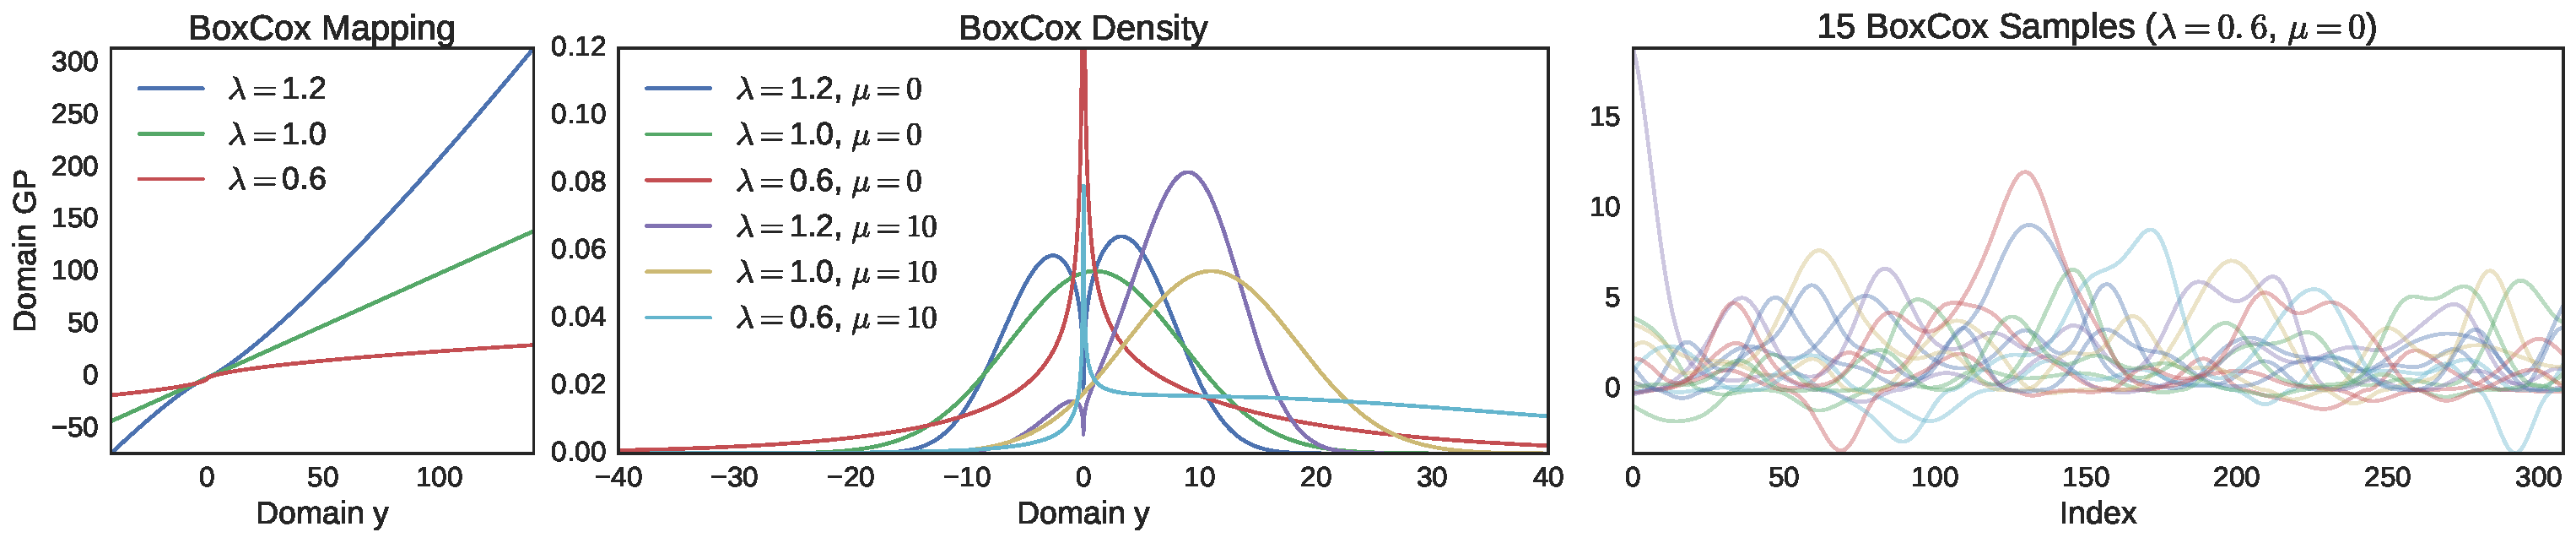
\includegraphics[width=1.0\textwidth]{boxcox_density_samples}\\
	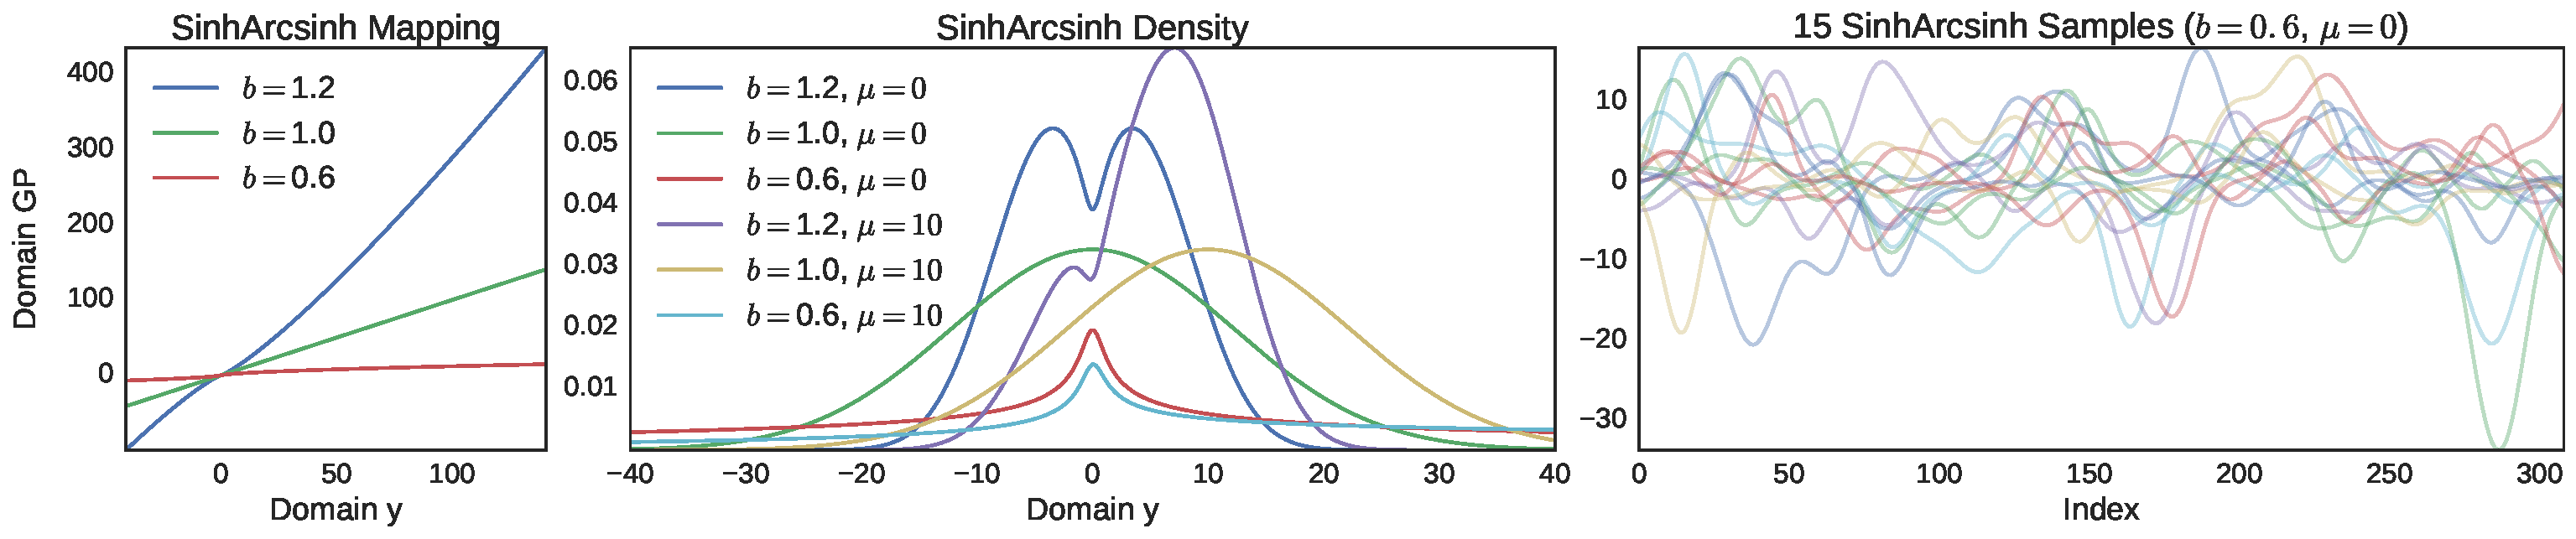
\includegraphics[width=1.0\textwidth]{sinharcsinh_density_samples} %scale=0.29, clip,trim=30 0 0 0
	\caption{Transformaciones elementales Box-Cox y Sinh-Asinh propuestas. Para todos los gráficos, \(\mu\) denota la media del GP basal \(x\). Arriba: la transformación de Box-Cox en la ecuación \eqref{eq:box-cox-trans}. Abajo: la transformación Sinh-Asinh en la ecuación \eqref{eq:sinharcsinh-trans}. Izquierda: las transformaciones. Centro: las densidades marginales inducidas. Derecha: muestras del GP deformado.}
	\label{fig:tgp_processes}
	%\vspace{-1em}
\end{figure*}

\subsection{Transformación Afín}

La transformación afín está dada por
\begin{equation}
	\label{eq:affine-trans}
	\varphi_{\text{afín}}(y) = a + by,
\end{equation}
para \(a, b \in \reals\), y se llama \emph{desplazamiento} (\emph{shift} en inglés) cuando \(b=1\) y \emph{escala} cuando \(a=0\). La transformación afín no proporcional ninguna capacidad mejorada para modelar por sobre los GP estándar, pues un GP transformado por \(\varphi_{\text{afín}}\) sigue siendo un GP con la media desplazada la varianza escalada. sin embargo, la deformación afín puede ser compuesta con otras funciones elementales para producir transformaciones expresivas.

\subsection{Transformaciones de Box-Cox}
\label{sec:BC_trans}
Una estrategia estándar en estadística para transformar observaciones no gaussianas positivas en unas \emph{parecidas a gaussianas} es aplicar la función logaritmo \(\varphi_{\log}(y) = \log(y)\). Este es el caso de procesos estocásticos con valores positivos y de colas pesadas \cite{aitchison1976lognormal}. Notemos que con la transformación logarítmica tanto la media \(m_x\) y la varianza \(\sigma_x^2\) del GP original \(x\) afectan a todos los momentos delproceso transformado \(y\). De forma explícita, el \(n\)-ésimo momento de \(y\) está dado por
\begin{equation}
	\mean_{y}[y^{n}] = \exp \bigl(nm_{x} + \tfrac{1}{2}n^{2} \sigma_{x}\bigr),
\end{equation}
lo que significa que una distribución con cola pesada para \(y\) se obtiene solo mediante la modificación de la media y la varianza del proceso original \(x\).

Una generalización de la transformación logarítmica es la transformación de Box-Cox \cite{boxcox,sakia1992box}, una función de potencias de un parámetro dada por
\begin{equation}
	\label{eq:box-cox-trans}
	\varphi_{\lambda}(y) = \frac{\sgn(y) \lvert y \rvert^{\lambda} - 1}{\lambda},
\end{equation}
donde \(\lambda \in \reals^{+}_{0}\). La función \(\varphi_{\lambda}\) se vuelve una de potencias para \(\lambda >0\), una transformación afín cuando \(\lambda = 1\), y la transformación logarítmica cuando \(\lambda = 0\), pues \(\varphi_{\lambda} \to \log(y)\) cuando \(\lambda \to 0\).

La transformación de Box-Cox tiene dos propiedades útiles. La primera es que su moda es \cite{powernormal}
\begin{align*}
	\mode(y) = \left[\frac{1}{2} \left(1 + \lambda m_x + \sqrt{(1 + \lambda m_x)^{2} + 4 \sigma_x^2 \lambda (\lambda - 1)}\right)\right]^{\frac{1}{\lambda}},
\end{align*}
donde \(m_x\) y \(\sigma_x^2\) son la media y la varianza del GP \(x\) respectivamente. Esta fórmula es particularmente útil para distribuciones asimétricas, donde es usual estimar la moda, no así la media o la mediana. La segunda propiedad es que el cálculo de momentos usando métodos numéricos, como la cuadratura de Gauss-Hermite \cite{gausshermite64}, se puede realizar con una precisión alta debido a la naturaleza polinomial de la transformación de Box-Cox. La figura \ref{fig:tgp_processes} (arriba) muestra diferentes transformaciones de Box-Cox con sus densidades marginales inducidas.

\subsection{Transformaciones hiperbólicas}
La distribución que resulta de tomar una variable aleatoria distribuida como \(\calN(0, 1)\) y aplicarle la transformación del seno hiperbólico inverso
\begin{align}
	\label{eq:arcsinh-trans}
	\varphi_{\asinh}(y) = a + b \asinh\left(\frac{y - c}{d}\right),
\end{align}
donde \(a, c \in \reals\) y \(b, d \in \reals^{+}\), se conoce como la distribución SU de Johnson \cite{johnsonsu} y tiene expresiones cerradas para la media y la varianza, dadas respectivamente por
\begin{align*}
	\mu_{\mathrm{SU}}			&= c - d \exp\left(\frac{b^{-2}}{2}\right) \sinh\Bigl(\frac{a}{b}\Bigr)\\
	\sigma_{\mathrm{SU}}^{2}	&= \frac{d^{2}}{2} \bigl(\exp\left(b^{-2}\right) - 1\bigr) \left[\exp\left(b^{-2}\right) \cosh\left(\frac{2a}{b}\right) + 1\right],
\end{align*}
y también para la asimetría y la curtosis \cite{johnsonsu}.

Otra transformación basada en fuciones hiperbólicas es la Sinh-Asinh \cite{Sinharcsinh}, en donde las funciones \(\asinh\), afín, y \(\sinh\) se componen como sigue:
\begin{equation}
	\label{eq:sinharcsinh-trans}
	\varphi_{\text{Sinh-Asinh}}(y) = \sinh(b\asinh(y) - a),
\end{equation}
en donde \(a, b \in \reals\). Esta distribución tiene expresiones explícitas para todos los momentos de \(y\), usando la función de Bessel modificada, e induce una distribución en donde los tercer y cuarto momentos pueden ser controlas a través de los parámetros \(a\) y \(b\). Esta distribución es simétrica si \(a = 0\), asimétrica positiva (resp. negativa) si \(a > 0\) (resp. \(a < 0\)), mesocúrtica si \(b = 1\), y leptocúrtica (resp. platicúrtica) si \(b > 1\) (resp. \(b < 1\)). Adicionalmente, la distribución cumple que \(0 < \lvert \mode(y) \rvert < \sinh(\lvert a \rvert / b)\) y \(\sgn(\mode(y)) = \sgn(a)\).

La figura \ref{fig:tgp_processes} (abajo) muestra transformaciones Sinh-Asinh con las marginales inducidas y muestras con un parámetro de asimetría \(a = 0\) y diferentes valores del parámetro de curtosis \(b\). Notemos que la media del GP basal, \(\mu\), también puede cambiar la asimetría de la distribución marginal inducida.

\section{¿Cómo Elegir las Transformaciones Elementales?}
\label{sec:choice_trans}

Así como en la gran mayoría de las estructuras profundas, la definición del número de capas y el tipo de neuronas está dada o por expertos o por prueba y error, done la interpretabilidad es una propiedad deseable \cite{representation_NN}. Esta habilidad es necesaria también en el caso cuando se escoge el kernel en máquinas de vectores de soporte o en procesos gaussianos (estudiado en \cite{duvenaud2013structure}). Recordemos que en los modelos de mezcla estándar (como un WGP) el usuario solo define el número de componentes, mientras que dentro del CWGP propuesto uno también necesita elgir los tipos y el orden de los elementos (en nuestro caso, funciones elementales). Esta sección guía la elección de las transformaciones elementales bajo dos escenarios, el primero siendo el caso cuando existe un conocimiento de expertos sobre los datos. En el segundo escenario, es decir, cuando no existe una información a priori de los datos, mostramos que se puede implementar un CWGP al concatenar múltiples instancias de una secuencia particular de funciones elementales (llamadas la \emph{capa Sinh-Asinh-Afín}), y mostramos que esta construcción tiene un rendimiento experimental atractivo. De esta forma, el CWGP puede ser considerado como una «caja negra» en donde, similar a las estructuras profundas, el usuario solo necesita escoger el número de capas. Ilustramos este concepto basado en la NLL (en la sección \ref{sub:sparse_trans}) y a través de un ejemplo de juguete (en la sección \ref{sub:replicating_wgp}), así como su robustez al sobreajustar y a través de datos reales en la sección \ref{sub:sunspots}.

\subsection{Cuando conocimiento previo de los datos está disponible}

Como mencionamos en la sección \ref{sec:BC_trans}, cuando los datos son estrictamente positivos, una práctica estándar es aplicar la transformación logarítmica. Es crítico que si se sabe que los datos tienen una cota inferior desconocida, uno puede componer la transformación logarítmica con la transformación \emph{shift} de la ecuación \eqref{eq:affine-trans} para encontrar el parámetro de \emph{shift} durante el entrenamiento. Encontrar una cota superior sigue un proceso análogo al reemplazar el \emph{shift} por una transformación afín, permitiendo así un escalamiento negativo. En este sentido, componer dos transformaciones afín-logarítmica nos permite encontrar las cotas inferior y superior simultáneamente.

Para relajar aún más la condición estricta de la cota (inferior) de la transformación logarítmica a una más permisiva, podemos reemplazar el logaritmo por la transformación de Box-Cox en la ecuación \eqref{eq:box-cox-trans}, en donde la permisividad de la cota está controlada por el parámetro \(\lambda\). Sumado a esto, si los datos son tales que su rango no está acotado, pero sí tienen una dispersión grande, entonces los datos siguen una distribución de cola pesada. Este fenómeno se puede modelar usando las transformaciones Asinh o Sinh-Asinh de las ecuaciones \eqref{eq:arcsinh-trans} y \eqref{eq:sinharcsinh-trans} respectivamente, pues dichas transformaciones permiten controlar la media y la varianza de la distribución, así como su asimetría y curtosis. Todas estas transformaciones pueden ser compuestas entre ellas para construir distribuciones más complejas, como en el caso de las distribuciones multimodales.

\subsection{Transformaciones compuestas \emph{sparse}}
\label{sub:sparse_trans}

Así como en cualquier modelo que involucre escoger un orden finito (como capas, neuronas, o componentes), se requiere que la adición de más funciones elementales en un CWGP tenga como resultado un desempeño monótonamente creciente. En particular, si uno considera un número innecesariamente grande de transformaciones elementales, es deseable que algunas de ellas \emph{se reviertan} a la función identidad (y así puedan ser removidas). Si, después de entrenar, algunas de las transformaciones se revierten a la identidad, diremos que la transformación compuesta es \emph{sparse}.

Cuando la intuición de las propiedades estadísticas de los datos es escasa, o incluso inexistente, un procedimiento recomendado es añadir de forma secuencial transformaciones que pueden revertirse a la identidad en caso de ser necesario. Notemos que si una transformación no es capaz de mejorar el desempeño y a la vez sí puede revertirse a la identidad, en efecto hará este. Este hecho se puede justificar basándonos en la NLL en la ecuación \eqref{eq:NLL}, en donde el término de ajuste a los datos permanece invariante, y el término de complejidad de la deformación contribuye a una NLL más baja. Sumado a esto, uno siempre puede escoger una distribución prior sobre los parámetros de la deformación para promover más deformaciones que estén cerca de la identidad. Finalmente, recordemos que, de las transformaciones propuestas, la Box-cox, la Sinh-Asinh y la afín pueden revertirse a la identidad, por lo que, bajo un conocimiento limitado sobre las propiedades subyacentes de los datos, recomendamos añadir estas componentes de forma iterativa hasta que el desempeño del modelo alcance una meseta. A continuación implementamos este concepto basados solo en las transformaciones Sinh-Asinh y afín en datos sintéticos.

\subsection{Descubrimiento de estructuras a través de transformaciones compuestas profundas}
\label{sec:experiments}

En los casos en que un conocimiento experto de los datos es escaso, el CWGP propuesto puede implementarse solo al concatenar múltiples instancias de las transformaciones elementales propuestas. Este procedimiento es usual y aceptado ampliamente en arquitecturas profundas generales \cite{bengio2009learning,Goodfellow-et-al-2016,DL_overview}. Para ilustrar esto, definamos primero la composición de las transformaciones Sinh-Asinh y Afín, de las ecuaciones \eqref{eq:arcsinh-trans} y \eqref{eq:affine-trans} respectivamente, llamada la \emph{capa SAL}\footnote{El acrónimo SAL viene de «Sinh-Asinh» y «Afín», done el uso de «L» viene de «lineal». Elegimos esta terminología para ser consistente con la parte experimental en la próxima sección.} dada por
\begin{equation}
	\label{eq:layer}
	l(y) = a + b \sinh(c \arcsinh(y) - d),
\end{equation}
donde \(a, b, c, d \in \reals\) son los únicos cuatro parámetros de la capa. Mostramos a continuación que solo al concatenar capas SAL podemos replicar la deformación «suma de tangentes hiperbólicas» implementada por un WGP \cite{snelson2004warped}, en la ecuación \eqref{eq:wgp}. La razón para evaluar el modelo propuesto en la aproximación del WGP es que se sabe que la suma de tangentes hiperbólicas es \emph{universal}, lo que significa que puede aproximar funciones continuas en cualquier grado de exactitud deseado en un intervalo cerrado.

Con la intención de obtener una comprensión intuitiva sobre la habilidad para modelar del enfoque por composiciones, el primer ejemplo ilustrativo es entrenar una transformación por composición de tres capas SAL, vía mínimos cuadrados, para replicar una mezcla de tres tangentes hiperbólicas. La figura \ref{fig:cwgp_flexible} muestra las transformaciones, derivadas, densidades y distribuciones de la verdad básica (el WGP, en azul) y la aproximación por composición de tres capas SAL (el CWGP, en verde). Notemos la similaridad punto a punto de las deformaciones, y que la masa de probabilidad se concentra alrededor de tres modas comunes en el dominio de \(y\).

\begin{figure}[h]
	\centering
	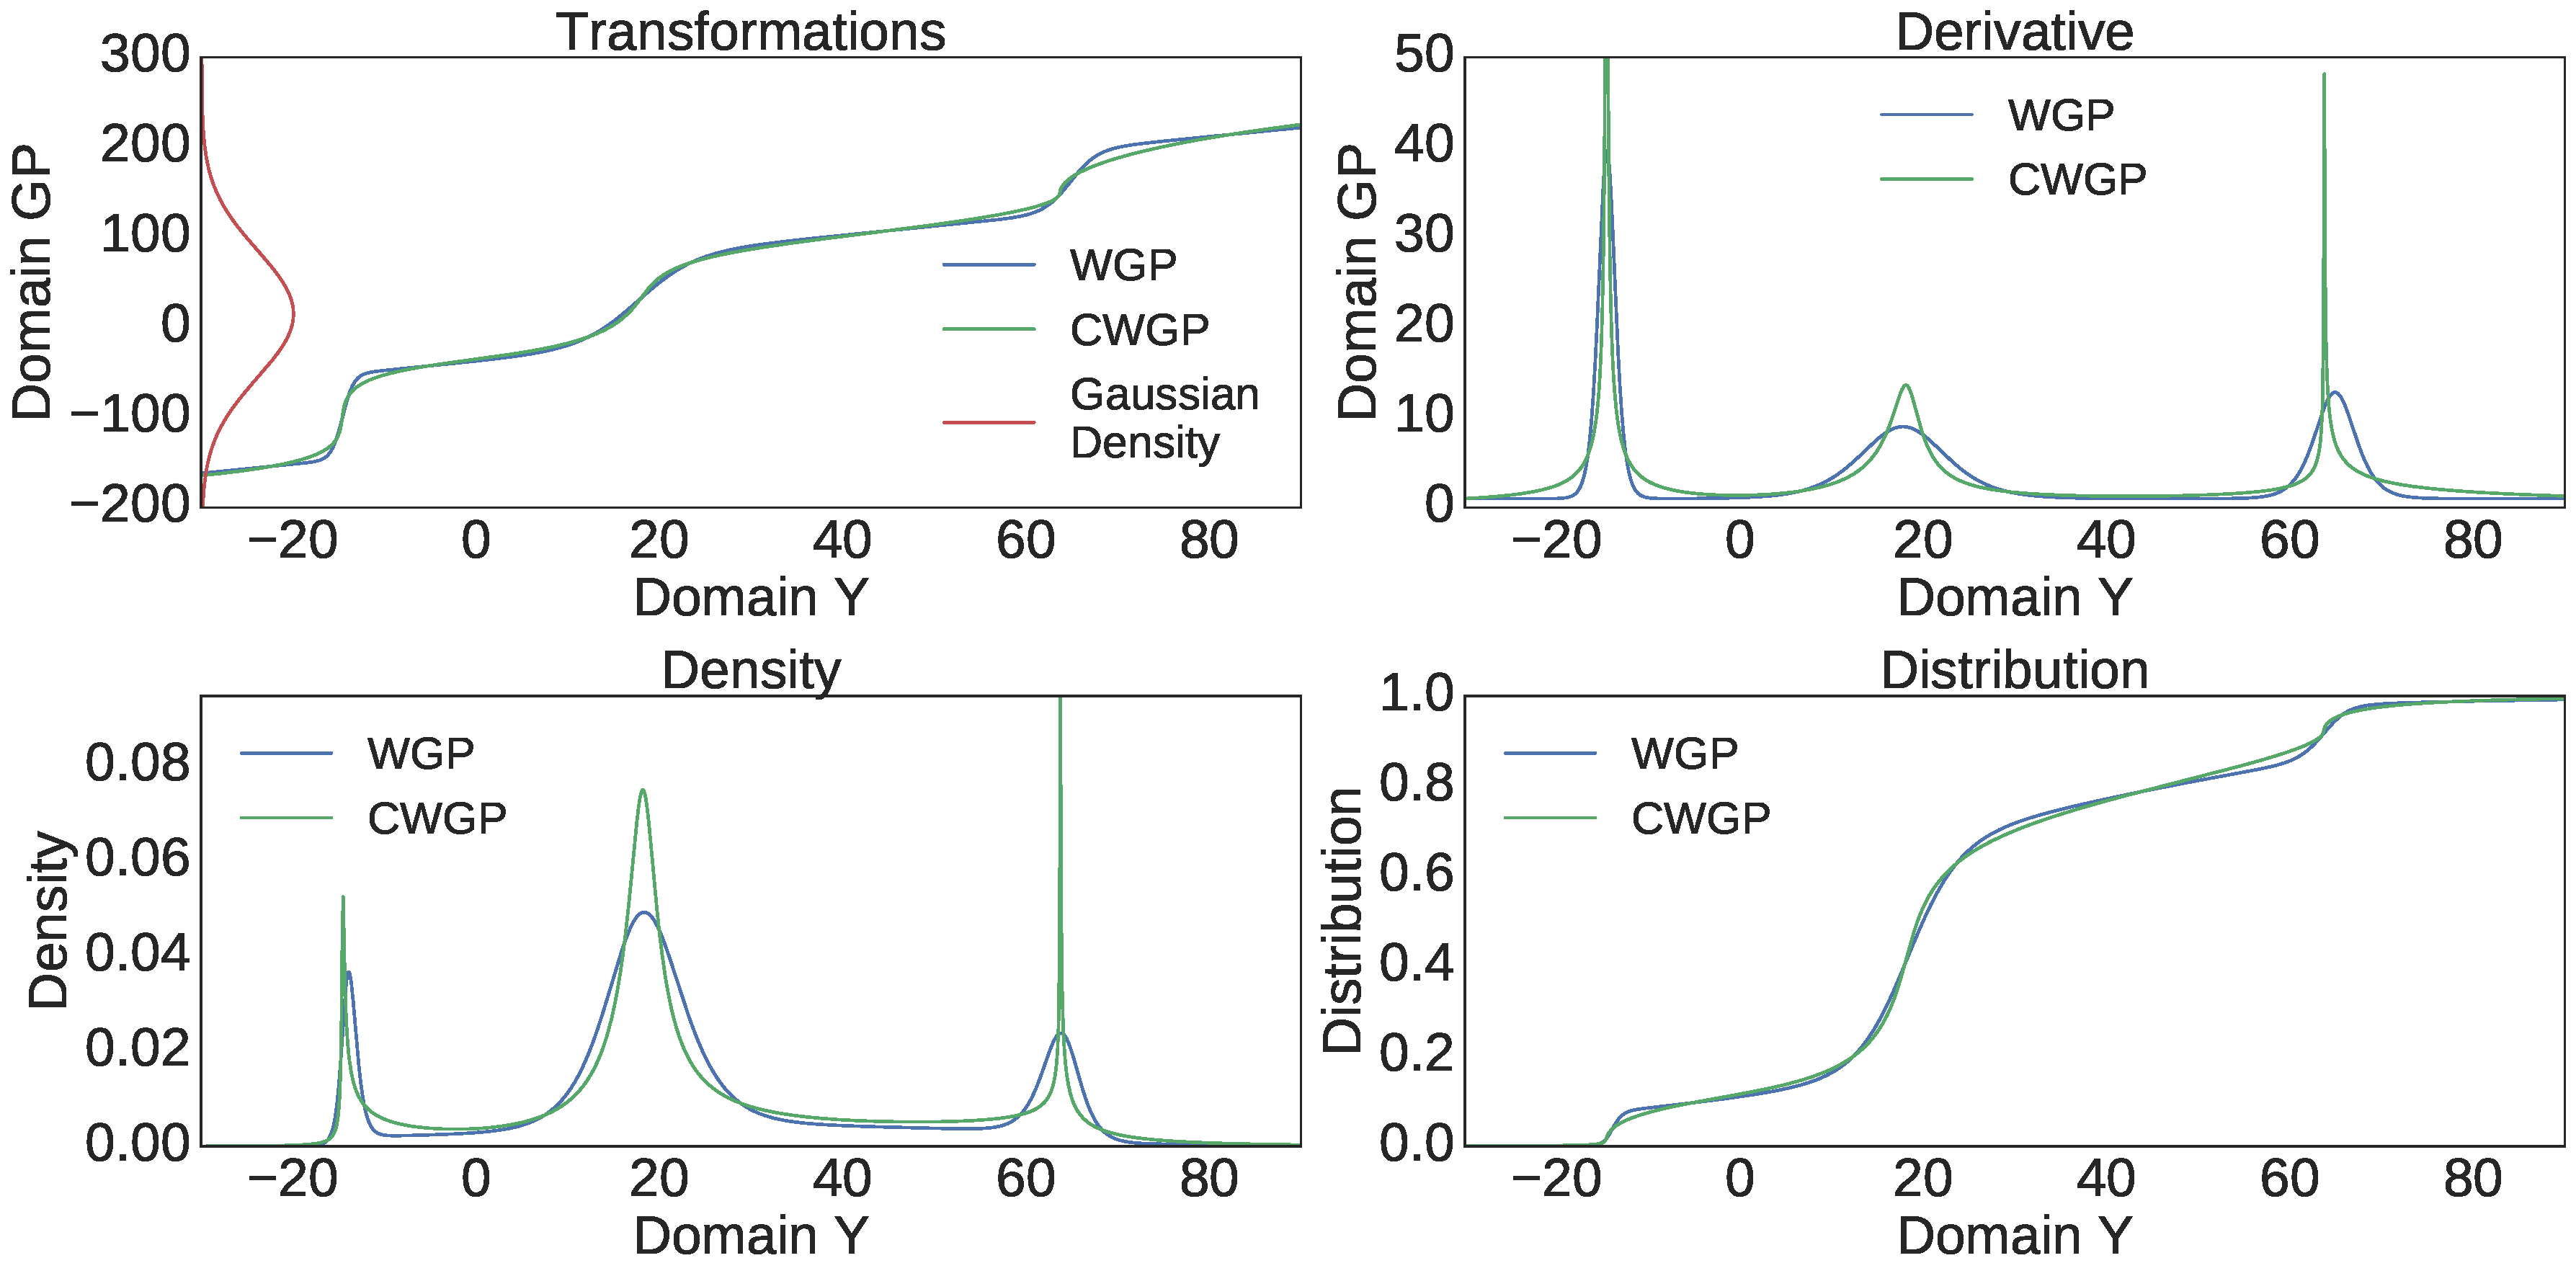
\includegraphics[width=0.8\textwidth]{cwgp_flexible}
	\caption{Aproximación de una deformación WGP (suma de tres tangentes hiperbólicas, en azul) usando el método por composición propuesto (tres capas SAL, en verde).}
	\label{fig:cwgp_flexible}
\end{figure}

Sobre la expresividad del enfoque por composición propuesto como una función del número de capas SAL consideradas, la figura \ref{fig:cwgp_blackbox1} muestra las distribuciones inducidas para un WGP con una deformación de cinco tangentes hiperbólicas (en azul) y aquellas de las aproximaciones compuestas usando de una a seis capas (en verde), ajustadas por mínimos cuadrados. Notemos cómo las distribuciones aprendidas por la transformación compuesta se vuelven indistinguibles de la verdad básica cuando el número de capas SAL crece.

\begin{figure}[h]
	\centering
	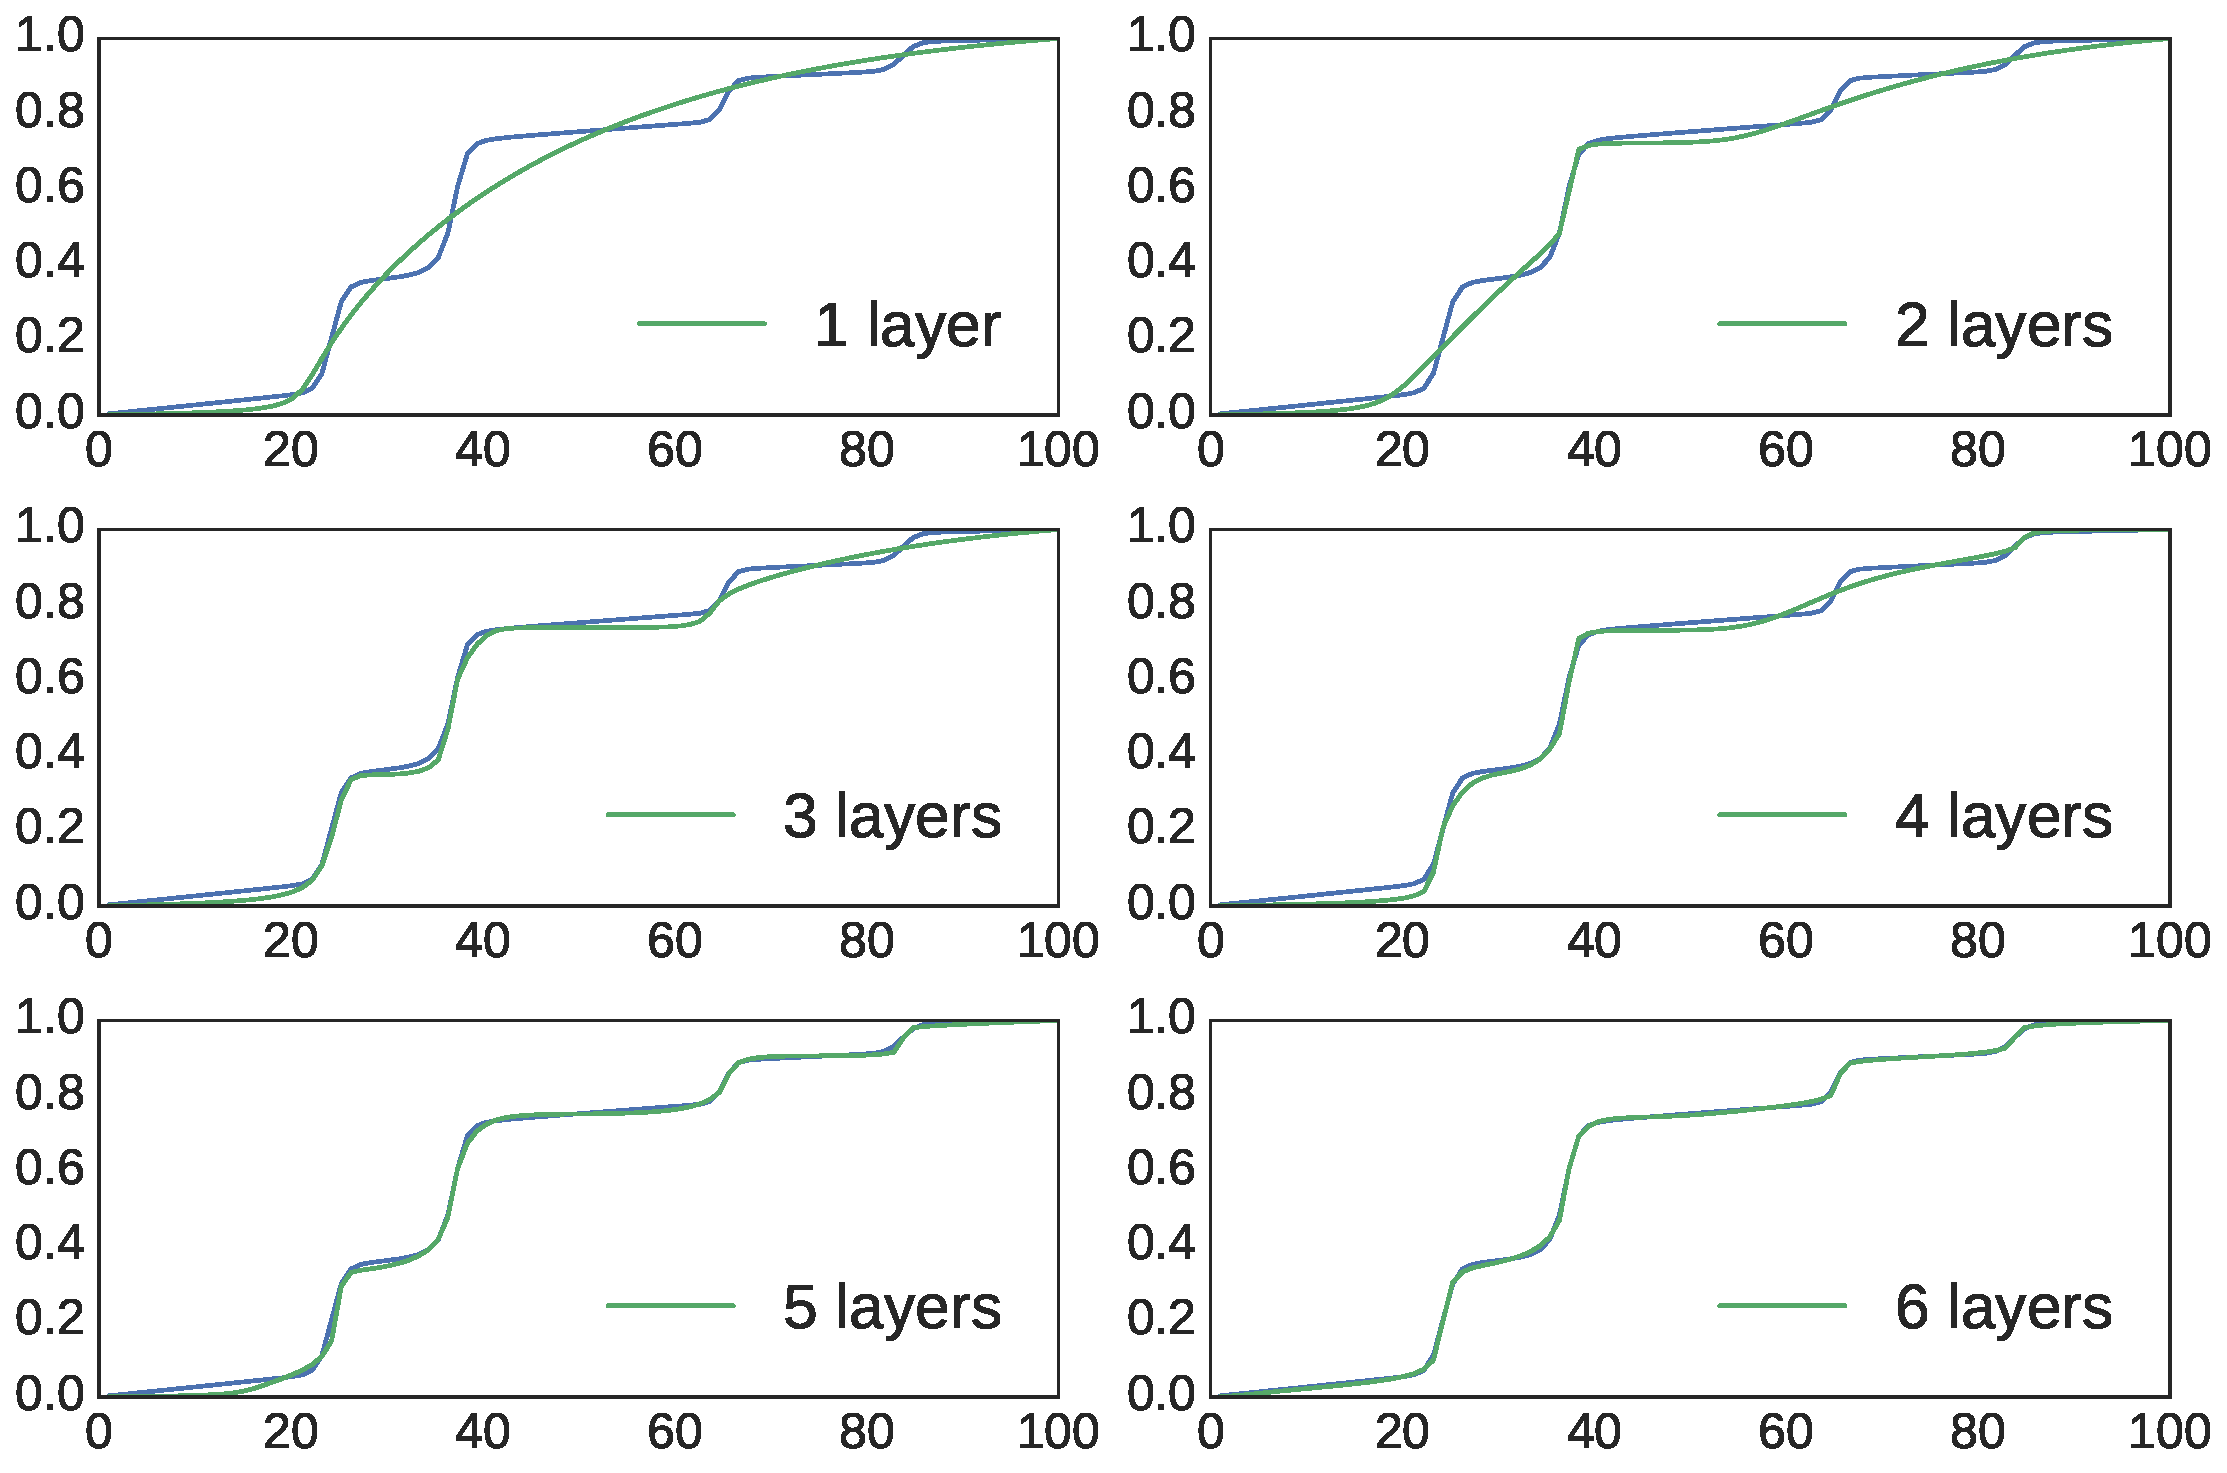
\includegraphics[width=0.7\textwidth]{cwgp_blackbox1}
	%\vspace{-1.5em}
	\caption{Aproximación CWGP de la distribución de un WGP con cinco tangentes hiperbólicas: la verdad básica (en azul) y las aproximaciones del CWGP (en verde), usando un número variable de capas SAL de la ecuación \eqref{eq:layer}.}
	\label{fig:cwgp_blackbox1}
	%\vspace{-1em}
\end{figure}

El cuadro \ref{tab:table_blackbox} reporta los errores de aproximación tanto para la transformación como para la distribución (deformada) resultante, usando las normas \(L_1\), \(L_2\) y \(L_\infty\) dadas por
%\begin{alignat*}{3}
%	e_1 &=||f_{\text{SoT}}-f_{\text{CT}}||_1 &&=\int_\reals|f_{\text{SoT}}(x)-f_{\text{CT}}(x)|dx\\
%	e_2 &=||f_{\text{SoT}}-f_{\text{CT}}||_2 &&=\sqrt{\int_\reals|f_{\text{SoT}}(x)-f_{\text{CT}}(x)|^2dx}\\
%	e_\infty &=||f_{\text{SoT}}-f_{\text{CT}}||_\infty &&=\sup_{x\in\reals}|f_{\text{SoT}}(x)-f_{\text{CT}}(x)|,
%\end{alignat*}
\begin{align*}
	e_1			&= \lVert f_{\mathrm{SdT}}-f_{\mathrm{TC}}\rVert_1 = \int_\reals \lvert f_{\mathrm{SdT}}(x) - f_{\mathrm{TC}}(x) \rvert \dd{x}\\
	e_2			&= \lVert f_{\mathrm{SdT}}-f_{\mathrm{TC}}\rVert_2 = \sqrt{\int_\reals \lvert f_{\mathrm{SdT}}(x) - f_{\mathrm{TC}}(x) \rvert^2 \dd{x}}\\
	e_\infty	&= \lVert f_{\mathrm{SdT}}-f_{\mathrm{TC}}\rVert_\infty = \sup_{x \in \reals} \lvert f_{\mathrm{SdT}}(x) - f_{\mathrm{TC}}(x) \rvert,
\end{align*}
donde \(f_{\mathrm{SdT}}\) denota a la transformación (o distribución) de la \emph{suma de tangentes hiperbólicas} del WGP, y \(f_{\mathrm{CT}}\) denota a aquellas de la \emph{transformación compuesta} propuesta. La figura \ref{fig:cwgp_blackbox2} muestra además las medidas de error antes descritas normalizadas con respecto al caso de una capa; notemos el desempeño monótono de la aproximación a medida de que el número de capas SAL aumenta.

\setlength{\tabcolsep}{4.4pt}
\begin{table}[h]
	\centering
	\begin{tabular}{crrrrrr}
		\toprule
		Capas	& Trans. \(L_1\)	& Trans. \(L_2\)	& Trans. \(L_\infty\)	& Dist. \(L_1\)	& Dist. \(L_2\)	& Dist. \(L_\infty\) \\
		\midrule
		1		& 1878.2			& 243.11			& 60.57					& 3.342			& 0.464			& 0.147 \\
		2		& 1147.7			& 151.86			& 33.77					& 2.232			& 0.292			& 0.107 \\
		3		&  845.14			& 124.80			& 37.19					& 1.628			& 0.192			& 0.047 \\
		4		&  582.53			&  83.71			& 27.34					& 1.464			& 0.184			& 0.041 \\
		5		&  319.64			&  41.33			& 15.28					& 0.793			& 0.115			& 0.057 \\
		6		&  147.78			&  19.95			&  6.48					& 0.316			& 0.042			& 0.015 \\
		7		&   91.64			&  15.71			&  8.32					& 0.174			& 0.025			& 0.011 \\
		\bottomrule
	\end{tabular}
	\caption{Aproximación «caja negra» de una deformación WGP con cinco tangentes hiperbólicas: medidas de error \(L_1\), \(L_2\) y \(L_\infty\) para las transformaciones y distribuciones inducidas, variando el número de capas.}
	\label{tab:table_blackbox} 
\end{table}

\begin{figure}[h]
	\centering
	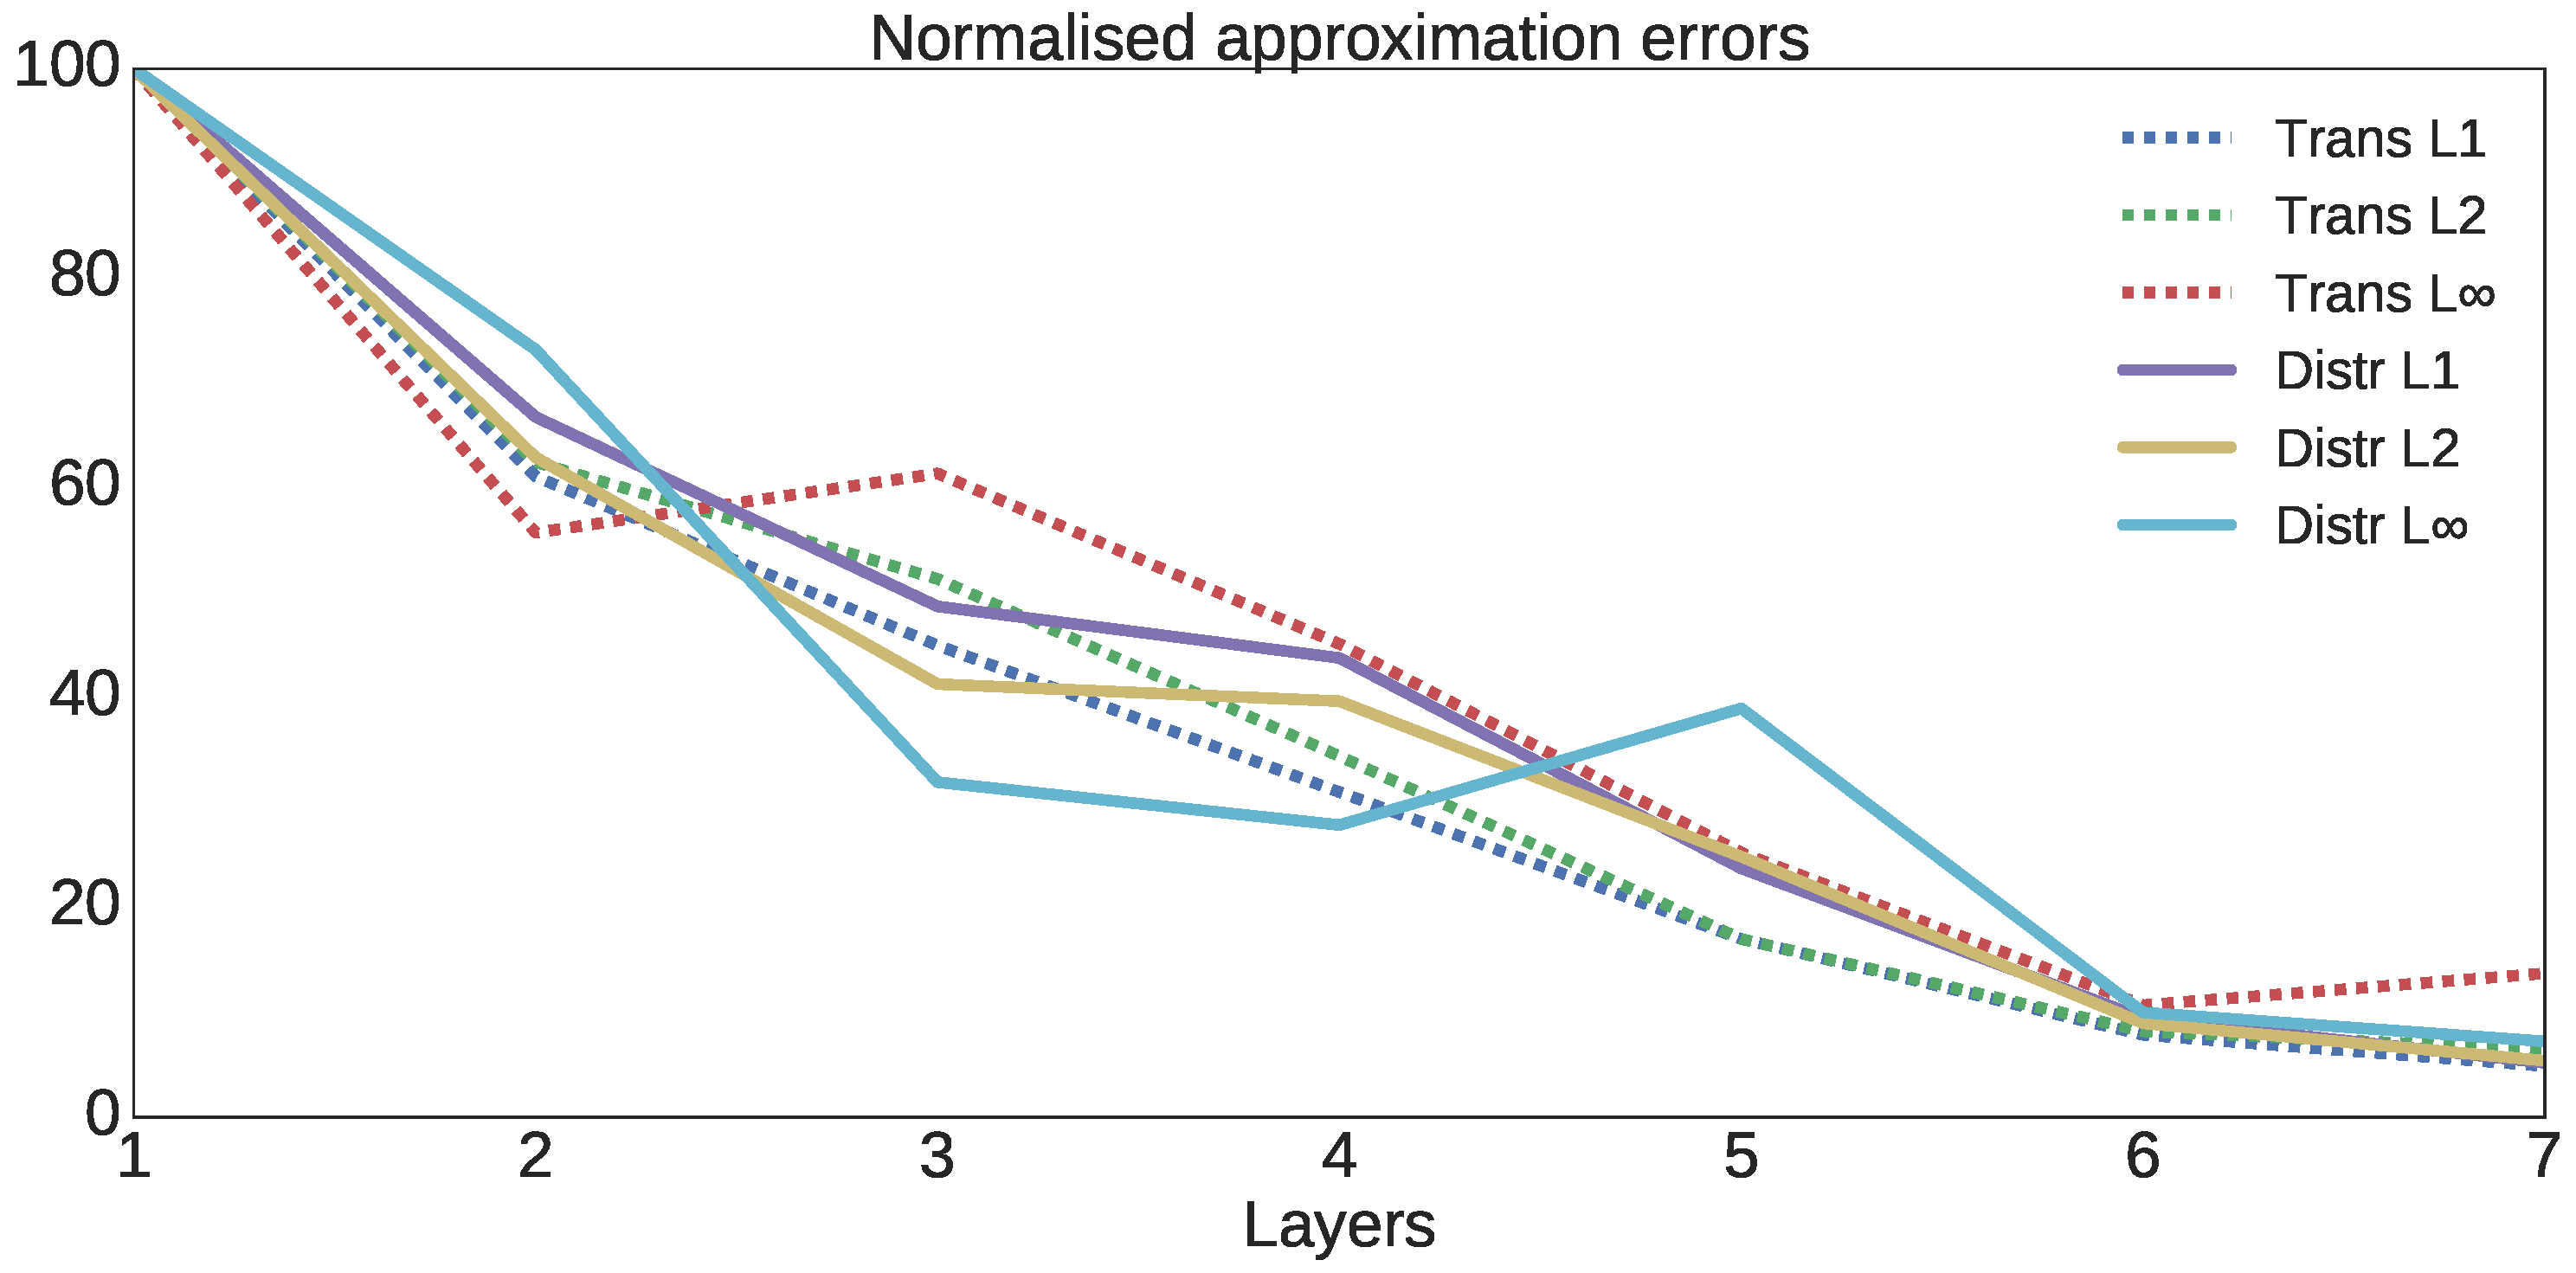
\includegraphics[width=0.7\textwidth]{cwgp_blackbox2}\\
	%\vspace{-1.5em}
	\caption{Representación de las medidas de error del cuadro \ref{tab:table_blackbox} normalizadas con respecto al error del caso de una capa.}
	\label{fig:cwgp_blackbox2}
	%\vspace{-1em}
\end{figure}


\comment{parrafo: falta la conclucion de capitulo, repasar lo mencionado, mencionar aplicaciones, limitantes, bondades y motivar la lectura en otros temas, mecionar temas similares o adyacentes}